\rchapter{Gyrokinetics}

\section{Introduction}

Particles in a plasma follow a complicated movement determined by electric and magnetic fields. The combination of the fields makes the particles move in a spiral motion around a guiding centre as shown by figure \ref{fig::guiding centre}.

\begin{figure}[ht]
 \centering
 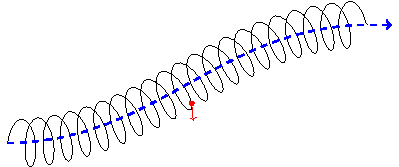
\includegraphics[width=.8\textwidth]{Figs/GyrokineticPrinciple}
 \caption{\label{fig::guiding centre}Path of a particle in a magnetic field and the guiding centre of that particle (shown in dashed blue)}
\end{figure}

This gyro-rotation is problematic for simulations as this motion means that the phase-space coordinates of the particle change rapidly. As a result, small time steps are required to obtain an accurate solution. Fortunately the high frequency gyro-rotation does not have an important effect on the low frequency physics demonstrated by the plasma, as a result if this motion can be rigorously removed from the equations of motion then the resulting equations which are less constrained can be used to analyse low frequency behaviour. In addition, the removal of this high frequency motion allows the reduction of the 6-D problem to a 5-D problem. This is the aim of gyrokinetics.

There are multiple methods used for finding the equations used in gyrokinetics (for example as described by Sugama et al \cite{Sugama2000}, Brizard \cite{BrizardGyro2000}, and others) which include some kind of coordinate transformations. The result of these transformations is that the coordinates are $(\vec{x},v_\parallel,\mu)$ where $\vec{x}$ is the position of the gyro centre, $v_\parallel$ is the velocity parallel to the time-independent background magnetic field $B_0$, and $\mu$ is the conserved magnetic moment. Normally there would also be a coordinate $\theta$ representing the gyroangle which is necessary to handle time-dependent fluctuations in the magnetic field, however the gyrokinetic transformations move these dependencies so that they are averaged which then removes them from the final equations. As a result the problem is reduced to five dimensions.

\section{Continuity Equation}

In the simulations, the plasma is described by a distribution function. This function describes the positions of a collection of identical particles of charge $q\neq 0$ and mass $m > 0$, immersed in a static magnetic field B(x). This value of this function is therefore conserved along particle trajectories\cite{MonteCarloBottino}:

\begin{equation}
 f\left(\vec{Z}\left(\vec{Z}_0,t\right),t\right) = f\left(\vec{Z}_0,t_0\right)
\end{equation}

The corresponding conservation equation is therefore defined as follows:

\begin{equation}
 \frac{d}{dt} f\left(\vec{Z}\left(\vec{Z}_0,t\right),t\right) = \dd{}{t}f\left(\vec{Z},t\right) + \underset{\alpha}{\sum} \frac{d\vec{Z}_\alpha}{dt}\dd{}{\vec{Z}}f\left(\vec{Z},t\right) = 0
\end{equation}

For the gyro-centre distribution function which is used for gyrokinetic theory, $f\in\reel_+$ and is a function of time $t\in\reel_+$ and of the phase space coordinates $\left(\vec{x},v_\parallel,\mu\right)$. This yields the following function:

\begin{equation}\label{eq::conservation general}
 \dd{}{t}f + \dot{\vec{x}}\cdot\grad f + \dot{v}_\parallel \dd{f}{v_\parallel} + \dot{\mu} \dd{f}{\mu} = 0
\end{equation}

The values of $\vec{u}=\dot{\vec{x}}$, $a_\parallel=\dot{v}_\parallel$, $M=\dot{\mu}$ can be determined using the Euler-Lagrange equations:

\begin{equation}
 \frac{d}{dt}\left(\dd{\mathcal{L}}{\dot{\vec{Z}}_\alpha}\right)-\dd{\mathcal{L}}{\vec{Z}_\alpha}=0
\end{equation}

where $\mathcal{L}$ is the Lie-transformed low-frequency particle Lagrangian obtained using gyrokinetic theory, defined (in SI units) as follows \cite{MonteCarloBottino}:

\begin{equation}
 L=\left(e\vec{A}+mv_\parallel\hat{b}\right)\cdot\dot{\vec{x}}+\frac{m\sqrt{4\pi}}{e\mu_0^{\frac{3}{2}}}\mu\dot{\theta}-H\left(\vec{x},v_\parallel\right)
\end{equation}

Although $\theta$ is not one of the gyrokinetic coordinates, it is a phase-space coordinate and as such can also be used to obtain useful equations. The Euler-Lagrange equation for $\theta$ is as follows:
\begin{align}
 \frac{d}{dt}\left(\frac{m\sqrt{4\pi}}{e\mu_0^{\frac{3}{2}}} \mu\right) + 0 = 0\\
 \dot{\mu} = 0\label{eq::mu dot def}
\end{align}

This implies that $M=\dot{\mu}=0$.

The Euler-Lagrange equation for $v_\parallel$ is as follows:

\begin{align}
 \frac{d}{dt}\Big(0\Big) - m \hat{b}\cdot\dot{\vec{x}}+\dd{H}{v_\parallel}=0\\
 \hat{b}\cdot\dot{\vec{x}}=\frac{1}{m}\dd{H}{v_\parallel}\label{eq::bxdotDefinition}
\end{align}

The Euler-Lagrange equation for $\vec{x}$ is as follows:

\begin{align}
 \frac{d}{dt}\left(e\vec{A}+mv_\parallel\hat{b}\right) - e\grad\left(A\cdot\dot{\vec{x}}\right)-mv_\parallel\grad\left(\hat{b}\cdot\dot{\vec{x}}\right) + \grad H = 0\\
 e\mathcal{J}_{\vec{A}}\dot{\vec{x}} + ma_\parallel\hat{b} + mv_\parallel\mathcal{J}_{\hat{b}}\dot{\vec{x}} - e\mathcal{J}_{\vec{A}}^T\dot{\vec{x}} - mv_\parallel\mathcal{J}_{\hat{b}}^T\dot{\vec{x}} + \grad H = 0\\
 \dot{v_\parallel}\hat{b} = \frac{e}{m}\left(\mathcal{J}_{\vec{A}}^T-\mathcal{J}_{\vec{A}}\right)\dot{\vec{x}} + v_\parallel \left(\mathcal{J}_{\hat{b}}^T-\mathcal{J}_{\hat{b}}\right)\dot{\vec{x}} - \frac{1}{m}\grad H
\end{align}

We now simplify the equations by introducing the following definitions:

\begin{gather}
 \vec{A}^*=\vec{A}+\frac{mv_\parallel}{e}\hat{b}\\
 \vec{B}^*=\grad\cross\vec{A}^* = \vec{B}+\frac{mv_\parallel}{e}\grad\cross\hat{b}
\end{gather}

Which leaves us with the equation:

\begin{align}\label{eq::EulerLagX}
 \dot{v_\parallel}\hat{b} = \frac{e}{m}\left(\mathcal{J}_{\vec{A}^*}^T-\mathcal{J}_{\vec{A}^*}\right)\dot{\vec{x}} - \frac{1}{m}\grad H
\end{align}

This equation can be simplified by remarking that $\left({\mathcal{J}_A^T}-{\mathcal{J}_A}\right)\vec{C} = \vec{C}\cross\left(\grad\cross\vec{A}\right)$ for all vector $\vec{C}$:

\begin{align*}
 \left[\vec{C}\cross\left(\grad\cross\vec{A}\right)\right]_i &= \varepsilon_{ijk}c_j\varepsilon_{klm}\partial_la_m\\
 &= \varepsilon_{kij}\varepsilon_{klm}c_j\partial_la_m\\
 &= \left(\delta_{il}\delta_{jm}-\delta_{im}\delta_{jl}\right)c_j\partial_la_m\\
 &= c_j\partial_ia_j - c_j\partial_ja_i\\
 &=\left({\mathcal{J}_A^T}_{ij}-{\mathcal{J}_A}_{ij}\right)c_j\\
 &=\left[\left({\mathcal{J}_A^T}-{\mathcal{J}_A}\right)\vec{C}\right]_i
\end{align*}

Equation \ref{eq::EulerLagX} is then written as follows:

\begin{align}
 \dot{v_\parallel}\hat{b} &= \frac{e}{m}\dot{\vec{x}}\cross\left(\grad\cross\vec{A}^*\right) - \frac{1}{m}\grad H\\
  &= \frac{e}{m}\dot{\vec{x}}\cross\vec{B}^* - \frac{1}{m}\grad H\label{eq::vbDefinition}
\end{align}

This expression can now be used to find a definition of $a_\parallel = \dot{v_\parallel}$. This is done by taking the dot product of the equation and $\hat{b}$:

\begin{align}
 \dot{v_\parallel}\vec{B}^*\cdot\hat{b} &= \frac{e}{m}\vec{B}^*\cdot\left(\dot{\vec{x}}\cross\vec{B}^*\right) - \frac{1}{m}\vec{B}^*\cdot\grad H\\
 \dot{v_\parallel} &= - \frac{\vec{B}^*}{mB_\parallel^*}\cdot\grad H\label{eq::a_parallel def}
\end{align}

where $B_\parallel^*=\hat{b}\cdot\vec{B}^*$.

The definition of $\vec{u}=\dot{\vec{x}}$ can also be found from equations \ref{eq::bxdotDefinition} and \ref{eq::vbDefinition} by taking the cross product of equation \ref{eq::vbDefinition} and $\hat{b}$ :

\begin{align}
 \dot{v_\parallel} \hat{b}\cross\hat{b} &= \frac{e}{m}\hat{b}\cross\left(\dot{\vec{x}}\cross\vec{B}^*\right) - \frac{1}{m}\hat{b}\cross\grad H\\
 0 &= \frac{e}{m}\left(\left(\hat{b}\cdot\vec{B}^*\right)\dot{\vec{x}}-\left(\hat{b}\cdot\dot{\vec{x}}\right)\vec{B}^*\right) - \frac{1}{m}\hat{b}\cross\grad H\\
 \frac{eB_\parallel^*}{m}\dot{\vec{x}} &= \frac{e}{m^2}\dd{H}{v_\parallel}\vec{B}^* + \frac{1}{m}\hat{b}\cross\grad H\\
 \dot{\vec{x}} &= \frac{1}{mB_\parallel^*}\dd{H}{v_\parallel}\vec{B}^* + \frac{1}{eB_\parallel^*} \hat{b}\cross\grad H\label{eq::u def}
\end{align}

The equations obtained using the Euler Lagrange equations (equations \ref{eq::mu dot def} \ref{eq::a_parallel def} \ref{eq::u def}) can now be substituted into equation \ref{eq::conservation general} to define the problem:

\begin{gather}
 \dd{}{t}f + \vec{u}\cdot\grad f + a_\parallel \dd{f}{v_\parallel} + \vec{M} \dd{f}{\mu} = 0\\
 \vec{u} = \frac{1}{mB_\parallel^*}\dd{H}{v_\parallel}\vec{B}^* + \frac{1}{eB_\parallel^*} \hat{b}\cross\grad H\\
 a_\parallel = - \frac{\vec{B}^*}{mB_\parallel^*}\cdot\grad H\\
 \vec{M}=0
\end{gather}

This expression depends on the Hamiltonian of the system which is defined using gyrokinetic theory as follows (in SI units) \cite{YamanPaper}: 

\begin{equation}
 H=\frac{1}{2}mv_\parallel^2 + \mu B(\vec{x})+e\langle\phi\rangle_g(t,\vec{x})
\end{equation}

This leaves the following definitions for the advection coefficients:

\begin{align}
 \vec{u} =& \frac{v_\parallel\vec{B}^*}{B_\parallel^*} + \frac{1}{eB_\parallel^*} \hat{b}\cross\left(\mu\grad B(\vec{x})+e\grad\phi\right) \label{eq::General u}\\
 a_\parallel =& - \frac{\vec{B}^*}{mB_\parallel^*}\cdot\left(\mu\grad B(\vec{x})+e\grad\phi\right)\label{eq::General a parallel}
\end{align}

\subsection{Cylindrical Geometry}

Generally the definition of the magnetic field used will be that used by Latu et al \cite{YamanPaper}:

\begin{align}
 \vec{B}=&\frac{B_0R_0}{R}\left(\zeta(r)\hat{\theta}+\hat{\varphi}\right) &&
 \zeta(r)=\frac{r}{q(r)R_0}
\end{align}

where $R_0$ is the major radius, $B_0$ is the toroidal magnetic field at the magnetic axis, $R(r,\theta) = R_\theta + r \cos\theta$ , and $q(r)$ is the classical safety factor in the large aspect ratio limit ($\frac{r}{R_0}\rightarrow 0$).

In the simplified case of a straight periodic cylinder, the toroidal angular variable $\hat{\varphi}$ is replaced by a straight variable $\hat{z} = R_0 \hat{\varphi}$, and R is taken to be equal to $R_0$. This leaves the following expression for the magnetic field:

\begin{align}
 \vec{B}=&B_0\left(\zeta(r)\hat{\theta}+\hat{z}\right) && \zeta(r)=\frac{\iota(r)r}{R_0}
\end{align}

where $\iota(r)=\frac{1}{q(r)}$.

The unit vector $\hat{b}$ is therefore defined as follows:

\begin{equation}\label{eq::magnetic unit}
\hat{b}=
\begin{cases}
 b_r=0\\
 b_\theta=\frac{s\zeta}{\sqrt{1+\zeta^2}}\\
 b_z=\frac{s}{\sqrt{1+\zeta^2}}
\end{cases}
\end{equation}

where $s=\text{sgn}(B_0)$.

This formulation has the advantage of simplifying equations \ref{eq::General u} and \ref{eq::General a parallel} as $\grad B=\vec{0}$. This can be proven using the fact that $B=\|\vec{B}\|$ and that it only depends on $r$. This means that $\left(\grad B\right)_\theta = \left(\grad B\right)_z = 0$ and $\left(\grad B\right)_r$ is determined below:

\begin{align*}
 \left(\grad B\right)_r =& \partial_r \sqrt{\underset{i}{\sum}B_i(r)^2}\\
 =&\frac{1}{B}\underset{i}{\sum} B_i(r) \partial_r B_i(r)\\
 =& \frac{1}{B}\left( B_\theta \partial B_\theta + B_z \partial_r B_z\right)\\
 =& \frac{1}{B}\left( \frac{s\zeta}{(1+\zeta^2)^{\frac{1}{2}}}\frac{s\partial_r\zeta}{(1+\zeta^2)^{\frac{3}{2}}} + \frac{s}{(1+\zeta^2)^{\frac{1}{2}}}\frac{-s\zeta\partial_r\zeta}{(1+\zeta^2)^{\frac{3}{2}}}\right)\\
 =& \frac{1}{B}\left( \frac{\zeta\partial_r\zeta}{(1+\zeta^2)^2}-\frac{\zeta\partial_r\zeta}{(1+\zeta^2)^2}\right)\\
 =& 0
\end{align*}

Equations \ref{eq::General u} and \ref{eq::General a parallel} can therefore be written as follows:

\begin{align}
 \vec{u} =& \frac{v_\parallel\vec{B}^*}{B_\parallel^*} + \frac{1}{B_\parallel^*} \hat{b}\cross\grad\phi\\
 a_\parallel =& - \frac{e\vec{B}^*}{mB_\parallel^*}\cdot\grad\phi
\end{align}

These equations are expressed in the orthogonal basis $(\hat{r},\hat{\theta},\hat{z})$. However for field-aligned expressions we are interested in objects which are parallel to the magnetic field. It is therefore important to identify these objects by including the magnetic unit vector $\hat{b}$ in the equations. In order to do this, the equations will now be expressed on the non-orthogonal basis $(\hat{r},\hat{\theta},\hat{b})$. These expressions can be found using the following definitions for an arbitrary vector $\vec{v}$:

\begin{equation*}
 \vec{v}=v_1\hat{r} + v_2\hat{\theta} + v_3\hat{z} \quad \quad \quad = v_1 \hat{r} + w_1\hat{\theta} + w_2\hat{b}
\end{equation*}
\vspace{-1.5em}
\begin{align*}
 w_1 =& \frac{v_2\hat{b}\cross\hat{\theta} + v_3\hat{b}\cross\hat{z}}{\hat{b}\cross\hat{\theta}}\\
 =& v_2 - v_3 \frac{b_\theta}{b_z}\\
 =& v_2 - v_3 \zeta\\
 w_2 =& \frac{v_3\hat{\theta}\cross\hat{z}}{\hat{\theta}\cross\hat{b}}\\
 =& \frac{v_3}{b_z}
\end{align*}

In order to express $a_\parallel$ in the non-orthogonal coordinates, $\vec{B}^*(x,v_\parallel)$ must first be expressed. In order to express $\vec{B}^*(x,v_\parallel)$, $\grad\cross\hat{b}$ is also needed:
\begin{align*}
 \grad\cross\hat{b} =& -\partial_rb_z\hat{\theta}+\frac{1}{r}\partial_r(rb_\theta)\hat{z}\\
 =& \left(\frac{s\zeta \zeta'}{\left(1+\zeta^2\right)^{\frac{3}{2}}}\right)\hat{\theta} + \left(\frac{s\zeta}{r\left(1+\zeta^2\right)^{\frac{1}{2}}} + \frac{s\zeta'}{\left(1+\zeta^2\right)^{\frac{3}{2}}}\right)\hat{z}\\
 =& \left(\frac{s\zeta \zeta'}{\left(1+\zeta^2\right)^{\frac{3}{2}}} - \frac{s\zeta^2}{r\left(1+\zeta^2\right)^{\frac{1}{2}}} - \frac{s\zeta'\zeta}{\left(1+\zeta^2\right)^{\frac{3}{2}}}\right)\hat{\theta}\\
 &+ \left(\frac{s\zeta}{r\left(1+\zeta^2\right)^{\frac{1}{2}}} + \frac{s\zeta'}{\left(1+\zeta^2\right)^{\frac{3}{2}}}\right)\frac{1}{b_z}\hat{b}\\
 =& - \frac{s\zeta^2}{r\left(1+\zeta^2\right)^{\frac{1}{2}}} \hat{\theta} + \left(\frac{\zeta}{r} + \frac{\zeta'}{1+\zeta^2}\right)\hat{b}
\end{align*}
where $\zeta'=\partial_r\zeta(r)$.

$\vec{B}^*(x,v_\parallel)$ can now be expressed:
\begin{align*}
 \vec{B}^*(x,v_\parallel) =& \vec{B}(x) + \frac{m}{e}v_\parallel \grad \cross \hat{b}(x)\\
 =& |B_0|\sqrt{1+\zeta^2}\hat{b}(x) + \frac{m}{e}v_\parallel \left[\frac{s\zeta\zeta'}{\left(1+\zeta^2\right)^{\frac{3}{2}}}\hat{\theta}\right.\\
 & \left.+ \frac{1}{r}\left(\frac{s\zeta}{\left(1+\zeta^2\right)^{\frac{1}{2}}} + \frac{rs\zeta'}{\left(1+\zeta^2\right)^{\frac{3}{2}}}\right)\hat{z}\right]
\end{align*}
\begin{align*}
 =& |B_0|\sqrt{1+\zeta^2}\hat{b}(x) + \frac{m}{e}v_\parallel \left[- \frac{s\zeta^2}{r\left(1+\zeta^2\right)^{\frac{1}{2}}} \hat{\theta} + \left(\frac{\zeta}{r} + \frac{\zeta'}{1+\zeta^2}\right)\hat{b}\right]\\
 =& - \frac{mv_\parallel}{e}\frac{s\zeta^2}{r\left(1+\zeta^2\right)^{\frac{1}{2}}} \hat{\theta} + \left[|B_0|\sqrt{1+\zeta^2} + \frac{mv_\parallel}{e}\left(\frac{\zeta}{r} + \frac{\zeta'}{1+\zeta^2}\right)\right]\hat{b}
\end{align*}

This leaves the following expression for $a_\parallel$:
\begin{align}
a_\parallel =& - \frac{e\vec{B}^*}{mB_\parallel^*}\cdot\grad\phi\nonumber\\
=& -\frac{e}{mB_\parallel^*}\left[-\frac{mv_\parallel}{e}\frac{s\zeta^2}{r^2\sqrt{1+\zeta^2}}\partial_\theta\phi + \left(|B_0|\sqrt{1+\zeta^2}\right.\right.\nonumber\\
&\left.\left.+\frac{mv_\parallel}{e}\left(\frac{\zeta}{r}+\frac{\zeta'}{1+\zeta^2}\right)\right)\hat{b}\cdot\grad\phi\right]\label{eq::a_parallel def cylinder}
\end{align}

In order to also express $\vec{u}$, $\hat{b}\cross\grad\phi$ must also be expressed:

\begin{align*}
 \hat{b}\cross\grad\phi =& \left(b_\theta \partial_z\phi - b_z \frac{\partial_\theta \phi}{r} \right)\hat{r} + b_z \partial_r\phi \hat{\theta} - b_\theta \partial_r \phi \hat{z}\\
 =& \left(b_\theta \partial_z\phi - b_z \frac{\partial_\theta \phi}{r} \right)\hat{r} + \left(b_z \partial_r\phi + \frac{b_\theta^2}{b_z} \partial_r \phi\right) \hat{\theta} - \frac{b_\theta}{b_z} \partial_r \phi \hat{b}\\
 =& \left[\frac{b_\theta}{b_z}\left(\hat{b}\cdot\grad\phi - b_\theta \frac{\partial_\theta\phi}{r}\right) - b_z \frac{\partial_\theta \phi}{r} \right]\hat{r} + \left(\frac{b_z^2 + b_\theta^2}{b_z} \right)  \partial_r\phi \hat{\theta} - \frac{b_\theta}{b_z} \partial_r \phi \hat{b}\\
 =& \left[\frac{b_\theta}{b_z}\hat{b}\cdot\grad\phi - \frac{1}{b_z} \frac{\partial_\theta \phi}{r} \right]\hat{r} + \frac{1}{b_z}   \partial_r\phi \hat{\theta} - \frac{b_\theta}{b_z} \partial_r \phi \hat{b}\\
\end{align*}

This leaves the following expression for $\vec{u}$:
\begin{align}
\vec{u} =& \frac{v_\parallel\vec{B}^*}{B_\parallel^*} + \frac{1}{B_\parallel^*} \hat{b}\cross\grad\phi\nonumber\\
=& \frac{1}{B_\parallel^*} \left[\left(\zeta\hat{b}\cdot\phi - \frac{s}{\sqrt{1+\zeta^2}}\frac{\partial_\theta\phi}{r}\right)\hat{r} \right.\nonumber\\
&+ \left(\frac{s}{\sqrt{1+\zeta^2}}\partial_r\phi - \frac{mv_\parallel^2}{e}\frac{s\zeta^2}{r\sqrt{1+\zeta^2}}\right)\hat{\theta}\nonumber\\
&+ \left.\left(|B_0|\sqrt{1+\zeta^2}v_\parallel + \frac{mv_\parallel^2}{e}\left(\frac{\zeta}{r} + \zeta'\frac{\zeta^2}{1+\zeta^2}\right)-\zeta \partial_r\phi\right)\hat{b}\right]\label{eq::u def cylinder}
\end{align}

In order to complete the definition, $B^*_\parallel$ is also expressed explicitly:
\begin{align}
 B^*_\parallel =& B^*_\theta b_\theta + B^*_z\nonumber\\
 =& |B_0|\sqrt{1+\zeta^2} + \frac{mv_\parallel}{e}\left(-\frac{\zeta^3}{r\left(1+\zeta^2\right)} + \frac{\zeta}{r} + \frac{\zeta'}{1+\zeta^2}\right)\nonumber \\
 =& |B_0|\sqrt{1+\zeta^2} + \frac{mv_\parallel}{e}\left(\frac{\zeta+\zeta'r}{r\left(1+\zeta^2\right)}\right)\label{eq::B parallel star cylinder}
\end{align}

For a torus to be effectively approximated by a straight cylinder, the major radius must be very large. As a result we let $\zeta(r)$ and $\zeta'(r)$ tend to 0. Applying this condition to equations \ref{eq::a_parallel def cylinder}, \ref{eq::u def cylinder}, and \ref{eq::B parallel star cylinder} gives the following expressions:

\begin{align}
 \vec{u} =& -\frac{1}{B_0}\frac{\partial_\theta\phi}{r} \hat{r} + \frac{1}{B_0}\partial_r\phi\hat{\theta} + v_\parallel \hat{b}\\
 a_\parallel =& -\frac{e}{m}\hat{b}\cdot\grad\phi
\end{align}

Thus equation \ref{eq::conservation general} can be written as follows:

\begin{gather}
 \partial_t f + \left(-\frac{1}{B_0}\frac{\partial_\theta\phi}{r} \hat{r}+\frac{1}{B_0}\partial_r\phi\hat{\theta} + v_\parallel \hat{b}\right)\cdot\grad f -\frac{e}{m}\hat{b}\cdot\grad\phi\,  \partial_{v_\parallel} f=0\\
 \partial_t f -\frac{1}{B_0}\frac{\partial_\theta\phi}{r} \partial_r f + \frac{1}{B_0}\partial_r\phi \frac{\partial_\theta\phi}{r} + v_\parallel \grad_\parallel f - \frac{e}{m}\grad_\parallel\phi\,  \partial_{v_\parallel} f=0
\end{gather}

To simplify the expression a Poisson bracket notation is introduced, defined as follows:
\begin{equation}
 \{\phi,f\}=-\frac{\partial_\theta\phi\partial_rf}{rB_0}+\frac{\partial_r\phi\partial_\theta f}{rB_0}
\end{equation}

This leaves the following final expression:

\begin{equation}\label{eq::Continuity Cylindrical}
 \partial_t f + \{\phi,f\} + v_\parallel \grad_\parallel f - \frac{e}{m}\grad_\parallel\phi\,  \partial_{v_\parallel} f=0
\end{equation}

\section{Quasi-Neutrality Equation}
% 
% Maxwell equations (in SI units):
% 
% \begin{align}
%  \grad \cdot \vec{E} &= \frac{\rho}{\varepsilon_0} &&= \frac{\underset{s}{\sum}q_sn_s}{\varepsilon_0} \label{Gauss Law}\\
%  \grad \cross \vec{E} &= -\frac{\partial \vec{B}}{\partial t}\label{Maxwell Faraday equation}\\
%  \grad \cdot \vec{B} &= 0 \label{Gauss Law Magnetism}\\
%  \grad \cross \vec{B} &= \mu_0 \vec{J} + \mu_0\varepsilon_0\dd{\vec{E}}{t} &&= \mu_0\underset{s}{\sum}j_s + \mu_0\varepsilon_0\frac{\partial \vec{E}}{\partial t}\label{Amperes Law}
% \end{align}
% 
% \begin{gather}
%  \vec{B} = \grad \cross \vec{A}\\
%  \vec{E} = -\grad\phi-\dd{\vec{A}}{t}
% \end{gather}
% 
% The Maxwell-Faraday equation (equation \ref{Maxwell Faraday equation}) and Gauss's law for magnetism (equation \ref{Gauss Law Magnetism}) can therefore be derived directly from the definitions of the potentials and the properties of the gradient and the rotational. The remaining two equations can be expressed as follows (using the fact that $\frac{1}{c^2}=\mu_0\varepsilon_0$):
% 
% \begin{gather}
%  \grad^2\phi + \dd{}{t}\left(\grad\cdot\vec{A}\right) = -\frac{\rho}{\varepsilon_0}\\
%  \left(\grad^2 \vec{A} - \frac{1}{c^2}\ddd{2}{A}{t}\right) - \grad\left(\grad\cdot \vec{A}+ \frac{1}{c^2}\dd{\phi}{t}\right)=-\mu_0\vec{J}
% \end{gather}
% 
% For a solution ($\phi$,$\vec{A}$) of the system any potential ($\phi'$,$\vec{A}'$) such that $\phi'=\phi-\dd{\lambda}{t}$, and $\vec{A}' = \vec{A}+\grad\lambda$ is also a solution. To ensure the unicity of the solution a gauge is chosen. A popular gauge is the Coulomb gauge which states that:
% 
% \begin{equation}
%  \grad\cdot\vec{A}=0
% \end{equation}
% 
% This simplifies the equations further leaving the following:
% 
% \begin{gather}
%  \grad^2\phi = -\frac{\rho}{\varepsilon_0}\\
%  \left(\grad^2 \vec{A} - \frac{1}{c^2}\ddd{2}{A}{t}\right) - \frac{1}{c^2}\dd{\grad\phi}{t}=-\mu_0\vec{J}
% \end{gather}
% 
% \begin{equation}
%  n_s = \int \hat{f}_s\delta([\vec{R}+\rho_s]-\vec{x})\mathcal{J}_s d^6Z
% \end{equation}
% 
% $\hat{f}_s$ is the the guiding-centre distribution defined as:
% 
% \begin{align*}
%  \hat{f}_s=&\bar{f}_s + \{\tilde{S},\bar{f}_s\} + \O{\varepsilon_g^2}\\
% 	  =&\bar{f}_s + \{\tilde{S},f_{M_s}  \} + \O{\varepsilon_g^2}
% \end{align*}
% 
% 
% Poisson bracket in gyro-centre coordinates:
% \begin{align}
%  \{F,G\}\equiv \frac{\Omega_s}{B_0}&\left(\dd{F}{\xi} \dd{G}{\mu}-\dd{F}{\mu}\dd{G}{\xi}\right) \nonumber\\
%   + \frac{B^*}{m_sB_\parallel^*}\cdot&\left(\grad F\dd{G}{u} - \dd{F}{u} \grad G\right) - \frac{c}{q_s B_\parallel^*}\vec{b}\cdot\grad F \cross \grad G
% \end{align}

Tronko et al. \cite{TronkoQuasiNeutrality} state the following (re-written in SI units):
\begin{equation}
 -\underset{sp}{\sum}\int dW \frac{1}{B_\parallel^*}\grad_\perp\cdot\left[ B_\parallel^* f_0 \frac{m}{B^2}\grad_\perp \phi_1\right] = \underset{sp}{\sum} q_s \int dW \mathcal{J}_0^{gc}f_1
\end{equation}

$B_\parallel^*$ is defined in equation \ref{eq::B parallel star cylinder} for cylindrical geometry. As above we take the limit $\zeta(r)\rightarrow0$ which leads $B_\parallel^*$ to converge towards the constant $|B_0|$. Given the dependencies of each element the equation can therefore be rewritten as follows:
\begin{align}
 -\underset{sp}{\sum} \grad_\perp\cdot\left[\left(\int dW f_0\right) \frac{m}{B^2}\grad_\perp \phi_1\right] = \underset{sp}{\sum} q_s \int dW \mathcal{J}_0^{gc}f_1\\
 -\underset{sp}{\sum} \grad_\perp\cdot\left[n_0 \frac{m}{B^2}\grad_\perp \phi_1\right] = \underset{sp}{\sum} q_s n_{1s}
\end{align}

Note that $n_{1s}=n_s-n_0$ and for adiabatic electrons $n_e=n_0 \exp\left(-q_e\frac{\phi-\langle \phi\rangle_r}{\kappa T_e}\right)$. The equation can therefore be written as:
\begin{equation}
 -\grad_\perp\cdot\left[\frac{\rho_{m0}}{B^2}\grad_\perp \phi\right] = q_i (n_i-n_0) + q_e n_0 \left(\exp\left(-q_e\frac{\phi-\langle \phi\rangle_r}{\kappa T_e}\right)-1\right)
\end{equation}
where $\rho_{m0}$ is the equilibrium mass density.

The linearisation of the exponential term leads to the following equation:
\begin{equation}
 -\grad_\perp\cdot\left[\frac{\rho_m}{B^2}\grad_\perp \phi\right] = q_i (n_i-n_0) - q_e^2 n_0 \frac{\phi-\langle \phi\rangle_r}{\kappa T_e}
\end{equation}

Dividing by $\varepsilon_0$ we obtain the following equation:
\begin{align}
 -\grad_\perp\cdot\left[\frac{\rho_{m0}}{\varepsilon_0B^2}\grad_\perp\phi\right] + \frac{q_e^2n_{0}}{\varepsilon_0\kappa T_e}\left[\phi-\langle\phi\rangle_f\right]=\frac{1}{\varepsilon_0}\rho_{c1}\\
 -\grad_\perp\cdot\left[\frac{\rho_{m0}}{\varepsilon_0B^2}\grad_\perp\phi\right] + \frac{1}{\lambda_D^2}\left[\phi-\langle\phi\rangle_f\right]=\frac{1}{\varepsilon_0}\rho_{c1}
\end{align}
where $\rho_{c1}$ is the charge perturbation density due to the ions and $\lambda_D=\sqrt{\frac{\varepsilon_0\kappa T_e}{q_e^2n_0}}$ is the electron Debye length.

In the case of non-adiabatic electrons, the electron contribution would take a similar form to the ionic contribution. This would be written as:
\begin{equation}
 -\grad_\perp\cdot\left[\frac{\rho_{m0}}{\varepsilon_0B^2}\grad_\perp\phi\right] + \frac{1}{\lambda_D^2}\left[\phi-\langle\phi\rangle_f\right]=\frac{1}{\varepsilon_0}\rho_{c1}
\end{equation}

as the electron contribution is absorbed by $\rho_{c1}$. The equation can also be simplified by removing the term $\langle\phi\rangle_f$. The final expression used will therefore be the following:
\begin{equation}\label{eq::quasi neutrality}
 -\grad_\perp\cdot\left[\frac{\rho_{m0}}{\varepsilon_0B^2}\grad_\perp\phi\right]+\frac{1}{\lambda_D^2}\left[\phi-\chi\cdot\langle\phi\rangle_f\right]=\frac{1}{\varepsilon_0}\rho_{c1}
\end{equation}

where $\chi$ is an optional parameter equal to either 0 or 1.